\documentclass[14pt]{extbook}
\usepackage{multicol, enumerate, enumitem, hyperref, color, soul, setspace, parskip, fancyhdr} %General Packages
\usepackage{amssymb, amsthm, amsmath, bbm, latexsym, units, mathtools} %Math Packages
\everymath{\displaystyle} %All math in Display Style
% Packages with additional options
\usepackage[headsep=0.5cm,headheight=12pt, left=1 in,right= 1 in,top= 1 in,bottom= 1 in]{geometry}
\usepackage[usenames,dvipsnames]{xcolor}
\usepackage{dashrule}  % Package to use the command below to create lines between items
\newcommand{\litem}[1]{\item#1\hspace*{-1cm}\rule{\textwidth}{0.4pt}}
\pagestyle{fancy}
\lhead{Progress Quiz 4}
\chead{}
\rhead{Version B}
\lfoot{9187-5854}
\cfoot{}
\rfoot{Spring 2021}
\begin{document}

\begin{enumerate}
\litem{
Determine the domain of the function below.\[ f(x) = \frac{4}{18x^{2} -54 x + 36} \]\begin{enumerate}[label=\Alph*.]
\item \( \text{All Real numbers except } x = a \text{ and } x = b, \text{ where } a \in [17.2, 19.3] \text{ and } b \in [35, 36.9] \)
\item \( \text{All Real numbers except } x = a, \text{ where } a \in [17.2, 19.3] \)
\item \( \text{All Real numbers except } x = a, \text{ where } a \in [-0.1, 1.8] \)
\item \( \text{All Real numbers except } x = a \text{ and } x = b, \text{ where } a \in [-0.1, 1.8] \text{ and } b \in [1.5, 2.8] \)
\item \( \text{All Real numbers.} \)

\end{enumerate} }
\litem{
Choose the equation of the function graphed below.
\begin{center}
    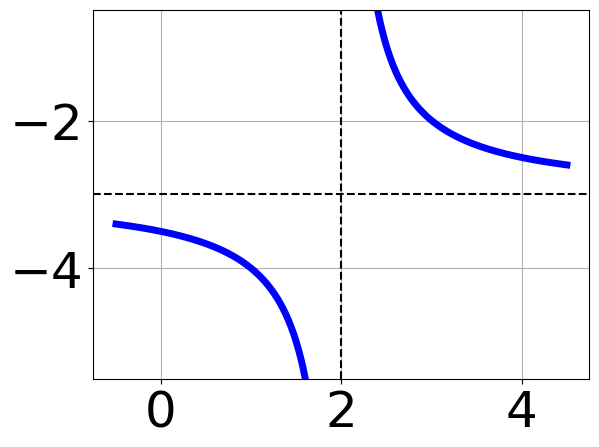
\includegraphics[width=0.5\textwidth]{../Figures/rationalGraphToEquationCopyB.png}
\end{center}
\begin{enumerate}[label=\Alph*.]
\item \( f(x) = \frac{-1}{(x - 3)^2} - 3 \)
\item \( f(x) = \frac{1}{x + 3} - 3 \)
\item \( f(x) = \frac{1}{(x + 3)^2} - 3 \)
\item \( f(x) = \frac{-1}{x - 3} - 3 \)
\item \( \text{None of the above} \)

\end{enumerate} }
\litem{
Solve the rational equation below. Then, choose the interval(s) that the solution(s) belongs to.\[ \frac{-56}{112x -28} + 1 = \frac{-56}{112x -28} \]\begin{enumerate}[label=\Alph*.]
\item \( x_1 \in [-0.6, -0.1] \text{ and } x_2 \in [-0.75,3.25] \)
\item \( x \in [0.25,1.25] \)
\item \( x_1 \in [-0.2, 1.3] \text{ and } x_2 \in [-0.75,3.25] \)
\item \( \text{All solutions lead to invalid or complex values in the equation.} \)
\item \( x \in [-0.6,-0.1] \)

\end{enumerate} }
\litem{
Determine the domain of the function below.\[ f(x) = \frac{5}{20x^{2} -8 x -12} \]\begin{enumerate}[label=\Alph*.]
\item \( \text{All Real numbers except } x = a, \text{ where } a \in [-15.4, -13.8] \)
\item \( \text{All Real numbers.} \)
\item \( \text{All Real numbers except } x = a \text{ and } x = b, \text{ where } a \in [-15.4, -13.8] \text{ and } b \in [15.4, 17.3] \)
\item \( \text{All Real numbers except } x = a \text{ and } x = b, \text{ where } a \in [-1, -0.2] \text{ and } b \in [0.8, 1.7] \)
\item \( \text{All Real numbers except } x = a, \text{ where } a \in [-1, -0.2] \)

\end{enumerate} }
\litem{
Choose the graph of the equation below.\[ f(x) = \frac{1}{(x - 1)^2} + 2 \]\begin{enumerate}[label=\Alph*.]
\begin{multicols}{2}\item 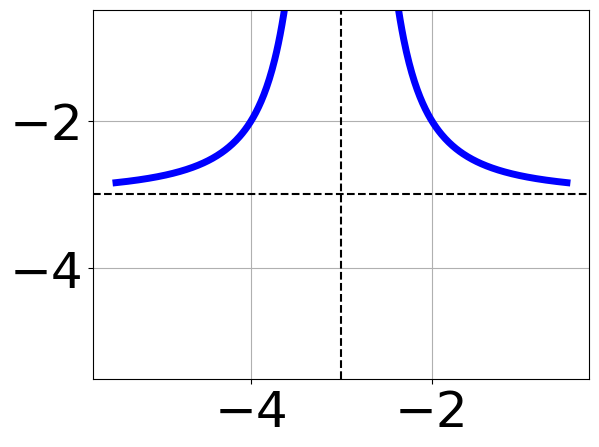
\includegraphics[width = 0.3\textwidth]{../Figures/rationalEquationToGraphCopyAB.png}\item 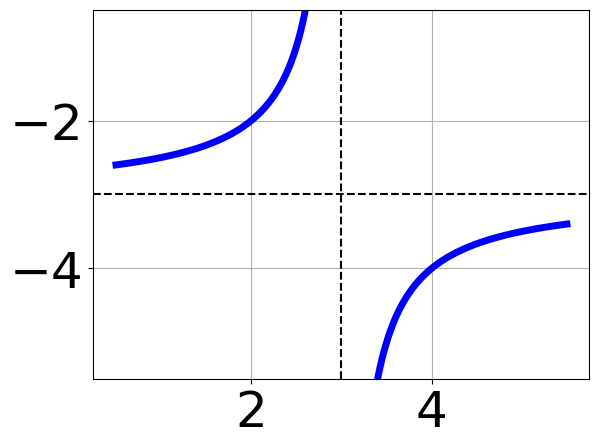
\includegraphics[width = 0.3\textwidth]{../Figures/rationalEquationToGraphCopyBB.png}\item 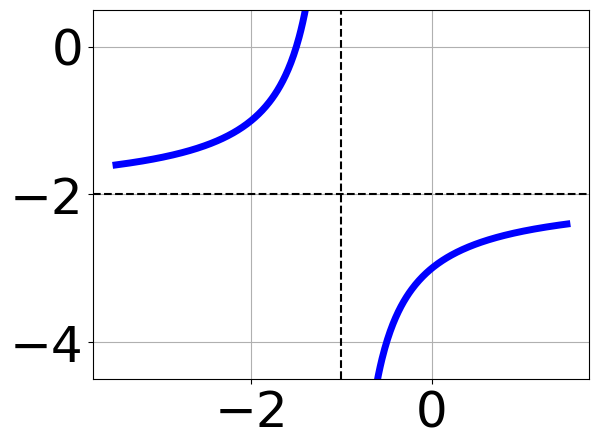
\includegraphics[width = 0.3\textwidth]{../Figures/rationalEquationToGraphCopyCB.png}\item 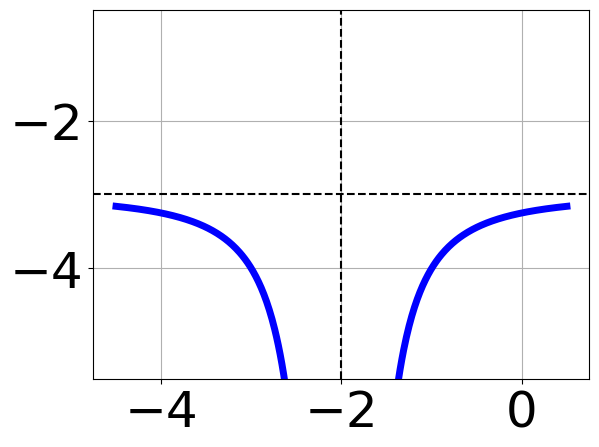
\includegraphics[width = 0.3\textwidth]{../Figures/rationalEquationToGraphCopyDB.png}\end{multicols}\item None of the above.
\end{enumerate} }
\litem{
Solve the rational equation below. Then, choose the interval(s) that the solution(s) belongs to.\[ \frac{-9}{-4x -8} + -2 = \frac{5}{-12x -24} \]\begin{enumerate}[label=\Alph*.]
\item \( x_1 \in [-1.67, 1.33] \text{ and } x_2 \in [3.33,5.33] \)
\item \( x \in [-0.67,1.33] \)
\item \( x \in [3.33,4.33] \)
\item \( x_1 \in [-1.67, 1.33] \text{ and } x_2 \in [-2.25,0.75] \)
\item \( \text{All solutions lead to invalid or complex values in the equation.} \)

\end{enumerate} }
\litem{
Solve the rational equation below. Then, choose the interval(s) that the solution(s) belongs to.\[ \frac{-3x}{6x -4} + \frac{-2x^{2}}{-18x^{2} +54 x -28} = \frac{2}{-3x + 7} \]\begin{enumerate}[label=\Alph*.]
\item \( \text{All solutions lead to invalid or complex values in the equation.} \)
\item \( x_1 \in [-0.51, 1.73] \text{ and } x_2 \in [-2.4,1.1] \)
\item \( x_1 \in [-0.51, 1.73] \text{ and } x_2 \in [3.4,6.2] \)
\item \( x \in [0.55,2.44] \)
\item \( x \in [3.75,6.76] \)

\end{enumerate} }
\litem{
Choose the equation of the function graphed below.
\begin{center}
    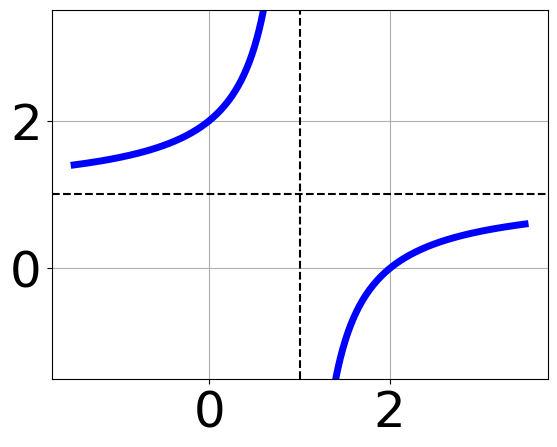
\includegraphics[width=0.5\textwidth]{../Figures/rationalGraphToEquationB.png}
\end{center}
\begin{enumerate}[label=\Alph*.]
\item \( f(x) = \frac{1}{(x + 1)^2} - 4 \)
\item \( f(x) = \frac{-1}{(x - 1)^2} - 4 \)
\item \( f(x) = \frac{-1}{x - 1} - 4 \)
\item \( f(x) = \frac{1}{x + 1} - 4 \)
\item \( \text{None of the above} \)

\end{enumerate} }
\litem{
Choose the graph of the equation below.\[ f(x) = \frac{1}{x - 3} + 3 \]\begin{enumerate}[label=\Alph*.]
\begin{multicols}{2}\item 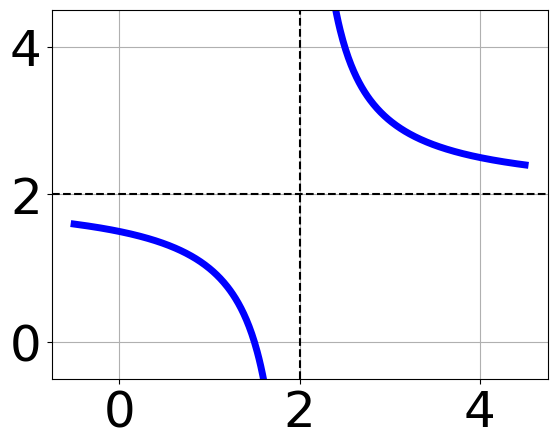
\includegraphics[width = 0.3\textwidth]{../Figures/rationalEquationToGraphAB.png}\item 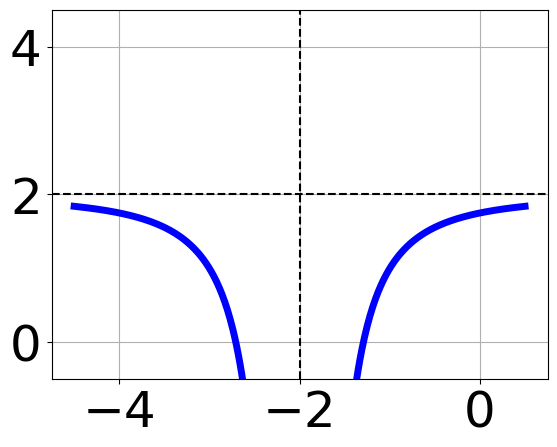
\includegraphics[width = 0.3\textwidth]{../Figures/rationalEquationToGraphBB.png}\item 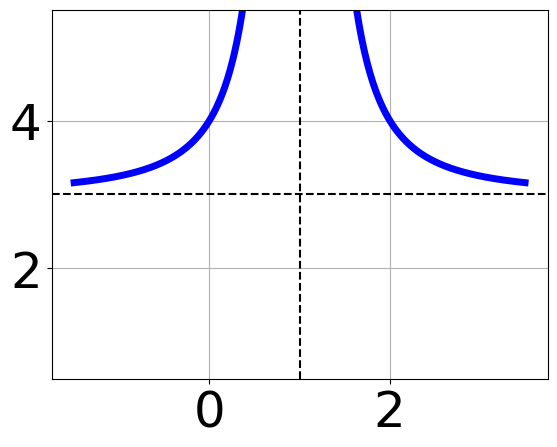
\includegraphics[width = 0.3\textwidth]{../Figures/rationalEquationToGraphCB.png}\item 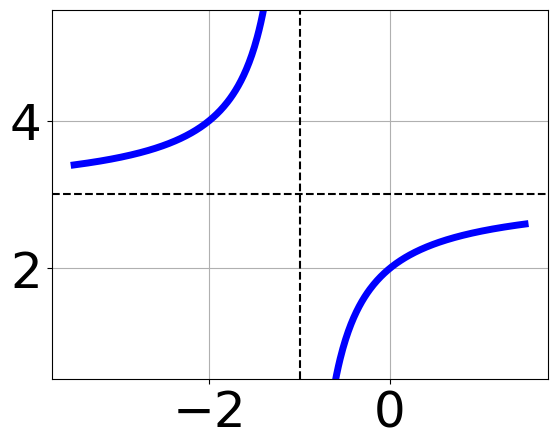
\includegraphics[width = 0.3\textwidth]{../Figures/rationalEquationToGraphDB.png}\end{multicols}\item None of the above.
\end{enumerate} }
\litem{
Solve the rational equation below. Then, choose the interval(s) that the solution(s) belongs to.\[ \frac{3x}{3x + 6} + \frac{-4x^{2}}{-6x^{2} -33 x -42} = \frac{5}{-2x -7} \]\begin{enumerate}[label=\Alph*.]
\item \( x \in [-1.48,-0.88] \)
\item \( x \in [-3.77,-3.24] \)
\item \( x_1 \in [-2.42, -1.94] \text{ and } x_2 \in [-2.39,-1.78] \)
\item \( x_1 \in [-2.42, -1.94] \text{ and } x_2 \in [-1.65,-1.12] \)
\item \( \text{All solutions lead to invalid or complex values in the equation.} \)

\end{enumerate} }
\end{enumerate}

\end{document}